\documentclass[class=scrbook, crop=false]{standalone}
\usepackage[subpreambles=true]{standalone}
\ifstandalone
    % WARNING: Proceed with caution!

% -----------------------------------------------------------------------------------
% For package standalone
% -----------------------------------------------------------------------------------
\usepackage{import}

% -----------------------------------------------------------------------------------
% Language and typeset
% -----------------------------------------------------------------------------------
\usepackage[ngerman, english]{babel}

\usepackage{subcaption}
% Umlauts and other special characters (UTF-8)
% \usepackage[utf8]{inputenc}
\usepackage{fontspec}
\setsansfont{Arial}
% \usepackage[T1]{fontenc}  % Enable accented characters and umlauts
% LuaLatex doesn't need fontenc and uses UTF-8
% \usepackage{lmodern}  % Font face


% --------------------------------------------------------------------------------
% Page formatting
% --------------------------------------------------------------------------------
% Change the header/footer for chapter beginnings and normal pages
\usepackage[automark,headsepline]{scrlayer-scrpage}

% The package provides an easy and flexible user interface to customize the page
% layout, implementing auto-centering and auto-balancing mechanisms
% WARNING: WHEN CHANGING BCOR (Binding correction), the cover needs reworking!...
\newcommand{\theBCOR}{15mm}  % Define binding correction
\usepackage[
    bindingoffset=\theBCOR,
    % showframe, % Show boxes which indicate margins and paddings
    bottom = 3.5cm, % Margins
      left = 2.5cm,
     right = 2.5cm
] {geometry}

% The package 'float' provides a container for document objects which can not be
% broken over pages, such as tables and figures
% Needed for table and figure indexes  
\usepackage{float}

% support for landscape layout
\usepackage{lscape}

% support of \tablenotes command to add notes under table
\usepackage{threeparttable}

% To allow drawing more professional tables
\usepackage{booktabs}

% --------------------------------------------------------------------------------
% Contents
% --------------------------------------------------------------------------------
% Vector graphics (for Cover page)
\usepackage{tikz} 

% Allows additional parameters when including images
\usepackage{graphicx}

% Roman font family for all headings
\addtokomafont{disposition}{\rmfamily}

% Set the line spacing to 1.5
\usepackage[onehalfspacing]{setspace}

% Improves overall text spacing
% http://www.khirevich.com/latex/microtype/
\usepackage[stretch=10]{microtype}

% Math symbols like mu outside the math environment
\usepackage{textcomp}

% A comprehensive (SI) units package∗
% For defining SI units
\usepackage[
    range-units=single,         % Formatting ranges with single unit indication: 1 - 2 m
    range-phrase=-,             % Phrase for range: 1 - 2 m vs 1 to 2 m
    separate-uncertainty=true,  % sets +- between value and uncertainty 
    multi-part-units=repeat     % In expressions with multiple values (multi part numbers) 
                                % the unit is printed each time: 1 mm x 1 mm
] {siunitx}
% https://tex.stackexchange.com/questions/124488/multi-part-numbers-and-units-in-siunitx

% Allows Sourcecodes with highlighting 
\usepackage{listings}

% This package provides user control over the layout of the three basic list
% environments: enumerate, itemize and description
\usepackage{enumitem}
\setlist{nosep} % Remove the vertical space between \item elements in all lists

% ToDo Notes
% \setlength{\marginparwidth}{2cm}
\usepackage{todonotes}
\setuptodonotes{inline, inlinepar}
\reversemarginpar  % Put ToDo notes on the binding's side
% \usepackage{soul} % Colorful ToDo notes

% Check out colors here http://latexcolor.com/
\usepackage{xcolor}

\usepackage{amsmath}    % alignment of equations

% --------------------------------------------------------------------------------
% Other elements
% --------------------------------------------------------------------------------
% Blindtext: Organic looking text dummy
\usepackage{blindtext}

% Hyperlinks within the document (PDF)
% "hidelinks" hides visual highlighting of links
\usepackage[hidelinks]{hyperref}

% Package for Glossary and Index (Acronyms are listed in a separate list) 
\usepackage[acronym, nogroupskip]{glossaries}[=v4.49] % groupskip: alphabetic grouping of entries

\usepackage{xltabular}   % <------- FOR glossaries

% Integration and management of bibliographies
\usepackage{csquotes}   % backend=biber in biblatex needs this package
\usepackage[
    style=ieee,   % style of the bibliography, entries are sorted in alphabetic order. "ieee" is another common style.
    backend=biber,      % based on package 'biber' 
    bibencoding=ascii   % ASCII Text encoding; may use "utf8" instead
] {biblatex}

% --------------------------------------------------------------------------------
%                               PATHS & FILES
% --------------------------------------------------------------------------------
% Fix paths for standalone compiling
\ifstandalone
    \def \home {..}
\else
    \def \home {.}
\fi

% Package: scrlayer-scrpage
% \def \stylePath {\home/settings+/style/page}
\input{\home/settings+/style/page}  % Load page style

% Package: graphicx
\graphicspath{{\home/images/}}  % Set path to images

% Package: listings
\input{\home/settings+/style/code.tex}  % Set path to style file
\lstset{inputpath={\home/code/}} % Default path to code listings

% Package: glossaries
\input{\home/settings+/style/symbols}  % Set path to symbols list style file
\input{\home/settings+/style/acronyms}  % Set path to acronym list style file
% -------------------------------------------------------------------------------
%               Listing of all Glossary and Acronym Entries 
%                           use as shown below
% -------------------------------------------------------------------------------

% ==== EXEMPLARY ENTRY FOR SYMBOLS LIST =========================================

% ==== EXEMPLARY ENTRY FOR ACRONYMS LIST ========================================
% \newacronym{#label}{#acronym}{#long_form}

% define new command for custom arconym entry with only two arguments
% fabricates an easier way to use \newacronym 
\newcommand{\acroX}[2]{\newacronym{#1}{#1}{#2}}
% \acroX{label and arconym}{long name}
% \acroX{CD}               {Compact Disk}

\newcommand{\acroY}[3]{\newacronym{#1}{#2}{#3}}
% \arcoY{label}{acronym}{long name}
% \acroY{CD}   {cd}     {Compact Disk}
 
\newacronym{AEP}{AEP}{Imbalance price}
\newacronym{aFRR}{aFRR}{Automatic Frequency Restoration Reserve}


\newacronym{reBAP}{reBAP}{Uniform imbalance price}
\newacronym{TSO}{TSO}{Transmission System Operator}
\newacronym{FCR}{FCR}{Frequency Containment Reserve}
\newacronym{mFRR}{mFRR}{Manual Frequency Restoration Reserve}
\newacronym{BRP}{BRP}{Balancing Responsible Party}
\newacronym{SB}{SB}{System Balance}
\newacronym{VRE}{VRE}{variable renewable energy}
\newacronym{ID1}{ID1}{intraday index ID1}
\newacronym{MAE}{MAE}{mean average error}
\newacronym{RMSE}{RMSE}{root mean squared error}
\newacronym{MSE}{MSE}{mean squared error}
\newacronym{CRPS}{CRPS}{continuous ranked probabililty score}
\newacronym{GCC}{GCC}{Grid Control Cooperation}
\newacronym{IC}{IC}{Continuous intraday}
\newacronym{VWAP}{VWAP}{volume-weighted average price}
\newacronym{VID}{VID}{traded volume within the intraday market}
\newacronym{ID AEP}{ID AEP}{Intraday Average Energy Price}
\newacronym{FRR}{FRR}{Frequency Restoration Reserve}
\newacronym{TFT}{TFT}{Temporal Fusion Transformer}
\newacronym{DLM}{DLM}{Dynamic Linear Model}
\newacronym{GB}{GB}{Gradient Boosting}
\newacronym{RF}{RF}{Random Forest}
\newacronym{ARIMAX}{ARIMAX}{Autoregressive Integrated Moving Average with eXogenous variables}
\newacronym{xLSTM}{xLSTM}{Extended Long Short-Term Memory}
\newacronym{DWD}{DWD}{Deutscher Wetterdienst}
\newacronym{ENTSO-E}{ENTSO-E}{European Network of Transmission System Operators for Electricity}
\newacronym{IDA1}{IDA1}{Intraday auction 1}
\newacronym{MOSMIX}{MOSMIX}{Model Output Statistics-MIX}
\newacronym{mLSTM}{mLSTM}{memory-optimized LSTM}
\newacronym{sLSTM}{sLSTM}{speed-optimized LSTM}

% ==== EXEMPLARY ENTRY FOR MAIN GLOSSARY ========================================

    % \newglossaryentry{policy}{name={Policy},description={Im geschäftlichen Bereich bezeichnet Policy eine interne Leit- bzw. Richtlinie, die formal durch das Unternehmen dokumentiert und über ihr Management verantwortet wird}}
    % \newglossaryentry{pcie}{name={PCI Express},description={PCI Express („Peripheral Component Interconnect Express“, abgekürzt PCIe oder PCI-E) ist ein Standard zur Verbindung von Peripheriegeräten mit dem Chipsatz eines Hauptprozessors. PCIe ist der Nachfolger von PCI, PCI-X und AGP und bietet im Vergleich zu seinen Vorgängern eine höhere Datenübertragungsrate pro Pin.}}
    % \newglossaryentry{realnumber}
  % Load glossary, symbol and acronyms list

% Package: biblatex
\addbibresource{\home/references/references.bib}  % Set path to bib resources

% Custom variables
\input{\home/settings+/variables}
% --------------------------------------------------------------------------------
%                                   OPTIONAL
% --------------------------------------------------------------------------------


% Simple arithmetic for LaTeX commands
% \usepackage{calc}

% Document Elements
% -------------------

% Index
% \usepackage{imakeidx}

% compact Lists
%\usepackage{paralist}

% visual improvements for citations
% \usepackage{epigraph}

% Create pseudo code
% https://www.overleaf.com/learn/latex/Algorithms
% \usepackage{algorithm}
% \usepackage{algorithmic}
%\usepackage[noend]{algpseudocode}

% Formatting
% -------------------
% Tweaks for scrbook, redefines commands of other packages
% \usepackage{scrhack}

% Intelligent space separator (nice for superscript?)
% \usepackage{xspace}

% Allows breaks within tables
%\usepackage{tabularx}

% Allows for page breaks in tables
% \usepackage{longtable}

% allows modifying of captions
% \usepackage{caption}

% Multiline comments
%\usepackage{verbatim}

% % Custom colors
% \definecolor{dartmouthgreen}{rgb}{0.05, 0.5, 0.06}

% IF you want to define unicode characters
% \DeclareUnicodeCharacter{0229}{\c{e}}
% \DeclareUnicodeCharacter{0306}{\u{Z}}


% Document elements
% ------------------------------------

% Table package
% \usepackage{booktabs}

% Pie diagram
% \usepackage{datapie}

% Side by Side images
% \usepackage{subcaption}

% For landscape tables
%\usepackage{pdflscape}
%\usepackage{afterpage}

% Graphics can be flow around by text
%\usepackage{wrapfig}

\fi

% ----------------------------------------------------------------------------
%                              Methodology
% ----------------------------------------------------------------------------
% Why do i use this data 
% What is this data
% Where is the data from
% How is the data presented
% When is the data available ?

\begin{document}

\chapter{Methodology} % Outline text
\label{Chapter::Methodology}
This chapter contains information about the data used for the Time Series prediction. 
The data can be separated into 3 thematic fields: weather data, market data and energy data.

In the following sections each data source will be described more in depth. 
This data is processed and filtered in chapter \ref{Chapter::Feature_Engineering}.

This chapter contains a more in depth overview about how the data was aquired and what information is available in the data used for the experiments. 
The data used for the experiments can be separated into 3 thematic fields: energy data, market data and weather data.
This chapter only provides a brief overview about the data sources. 

    
\section{Energy Data}
\label{Section::Energy_Data}

% Why do i use this data 
% What is this data
% Where is the data from
% How is the data presented
% When is the data available ?

The data used in this thesis is sourced from Netztransparenz and the ENTSO-E Transparency Platform.
The target variable, along with several additional explanatory variables, is obtained from these platforms.

Netztransparenz provides detailed information on the imbalance price and imbalance volumes, which are central to the prediction objective.
This data is available both operational and quality-assured.
The quality-assured data is available about 18 days after the operational data. 

ENTSO-E supplies load and generation data, including both measured values and forecasts, for the German electricity market.
Additionally, specific generation data is available for onshore wind, offshore wind, and solar photovoltaic technologies.
The data covers the German bidding zone exclusively, as the prediction task focuses solely on the German electricity market.
The forecast is done at 18:00 on the previous day. 
The time resolution of all datasets is quarter-hourly.
The period under study spans from the 21st of june 2022 to 31st of december 2024.

All datasets are accessed and downloaded via publicly available APIs, enabling automated and reproducible data collection.
An overview about all variables used by these data sources can be found in \ref{Table::Energy_Data_Netztransparenz} and \ref{Table::Energy_Data_Entsoe}.

A more detailed description of the preprocessing steps, feature engineering, and exploratory data analysis will be provided in later sections.

\begin{table}[]
\begin{tabular}{l|l|l|l}
 Data Source & Variable &  Time Resolution & Availability  \\\hline
 Netztransparenz & reBAP & 15 min & Real-time with 30 minutes delay \\
 Netztransparenz & NRV-saldo & 15 min & Real-time with 30 minutes delay \\
 Netztransparenz & Activated PRL & 15 min & Real-time with 30 minutes delay \\
 Netztransparenz & Activated SRL & 15 min & Real-time with 30 minutes delay \\
 Netztransparenz & SRL optimization & 15 min & Real-time with 30 minutes delay \\
 
\end{tabular}
\caption{Variables used from netztransparenz}
\label{Table::Energy_Data_Netztransparenz}
\end{table}

\begin{table}[]
\begin{tabular}{l|l|l|l}
 Data Source & Variable &  Time  & Availability  \\
 &&Resolution&\\\hline
 Entso-E & Load forecast & 15 min  & 12:00 d-1 \\
 Entso-E & Load actual & 15 min  & Real-time with max 1 h delay \\
 Entso-E & Wind onshore forecast & 15 min  & 18:00 d-1\\
 Entso-E & Wind offshore forecast & 15 min & 18:00 d-1 \\
 Entso-E & Solar forecast & 15 min & 18:00 d-1 \\
 Entso-E & Wind onshore actual generation & 15 min  & Real-time with max 1 h delay\\
 Entso-E & Wind offshore actual generation & 15 min & Real-time with max 1 h delay \\
 Entso-E & Solar actual generation & 15 min & Real-time with max 1 h delay \\
 Entso-E & Other renewable actual generation & 15 min & Real-time with max 1 h delay \\
 Entso-E & Hydro water reservoir actual generation & 15 min & Real-time with max 1 h delay \\
 Entso-E & Run of river actual generation & 15 min & Real-time with max 1 h delay \\
 Entso-E & Hydro pumped storage actual generation & 15 min & Real-time with max 1 h delay \\
 Entso-E & Hydro pumped consumption & 15 min & Real-time with max 1 h delay \\
 Entso-E & Lignite actual generation & 15 min & Real-time with max 1 h delay \\
 Entso-E & Fossil gas actual generation & 15 min & Real-time with max 1 h delay \\
 Entso-E & Fossil hard coal actual generation & 15 min & Real-time with max 1 h delay \\
 Entso-E & Fossil oil actual generation & 15 min & Real-time with max 1 h delay \\
  
\end{tabular}
\caption{Variables used from ENTSO-E}
\label{Table::Energy_Data_Entsoe}
\end{table}

\section{Market Data}
\label{Section::Market_Data}

The market data used in this thesis is provided by Energy-Charts \ref{EnergyCharts}.


Out of the data provided on the website, the prices for Day Ahead Auction, average intraday price, as well as intraday index 1 (ID1) and intraday index 3 (ID3) are used. 
More information about the used variables can be found in table \ref{Table::Market_Data}.

Each intraday index represents the volume-weighted average price of the trades during a certain period. 
While ID1 only considers trades that happened up to 1 hour before gate closure, ID3 considers trades up to 3 hours before gate closure time.
The variable Intraday continuous average is the volume-weighted average price of all trades that happened on the intraday market. 
This will be called ID FULL going further.

As described in \ref{Section::Imbalance_Price} one of the imbalance price modules is tied to the recent market situation.	

    
\begin{table}[]
\begin{tabular}{l|l|l|l}
 Data Source & Variable &  Time Resolution & Availability  \\\hline
 Energy-Charts & Hourly Spot price& 1 h& 12:00-15:00 d-1 \\
 Energy-Charts & Intraday auction 1 price & 1h & ?? ? ?? ?? ?\\
 Energy-Charts & Intraday Index 1 & 15 min &  00:00 d+1\\
 Energy-Charts & Intraday Index 3 & 15 min &  00:00 d+1\\
 Energy-Charts & Intraday Contiuous Average & 15 min &  00:00 d+1\\
   
\end{tabular}
\caption{Variables used from Energy-Charts}
\label{Table::Market_Data}
\end{table}

\section{Weather data}
\label{Section::Weather_Data}

The weather data used for the prediction of the imbalance price is obtained from the German Weather Service (DWD).
The dataset includes both measured weather observations and forecasted weather variables, with a time resolution of 1 hour.

Measured weather data is made available approximately one hour after observation, while weather forecasts cover a forecast horizon of up to 10 days into the future.

Since the generation of variable renewable energy (VRE) is highly dependent on weather conditions, the incorporation of weather data is essential for accurate modeling.
The data is aggregated from 16 weather stations distributed across Germany.
A complete list of the selected weather stations is provided in Appendix \ref{List::Weather_Stations}, and their geographic locations are illustrated in Figure \ref{fig::weather_stations}.

The full range of available weather variables for the measurements is summarized in Table \ref{Table::DWD_Measurement_Parameters}.
An overview about all available forecast variables can be found in the appendix (table \ref{Table::DWD_MOSMIX_Parameters}).
For the prediction task, a selected subset of forecast variables is used, as detailed in Table \ref{Table::DWD_MOSMIX_Parameters_Small}.


More information about how the data is handled will be discussed in section \ref{Section::Feature_Engineering}


\begin{table}[]
\begin{tabular}{l|l}
Parameter & Description \\\hline
DD & Wind direction\\
FF & Wind speed\\
FX1 & Maximum wind gust within the last hour\\
N & Total cloud cover\\
N05 & Cloud cover below 500 ft.\\
Neff & Effective cloud cover\\
Nh & High cloud cover (>7 km)\\
Nl & Low cloud cover (lower than 2 km)\\
Nm & Midlevel cloud cover (2-7 km)\\
RR1c & Total precipitation during the last hour consistent with significant weather\\
Rad1h & Global Irradiance\\
SunD1 & Sunshine duration during the last Hour\\
T5cm & Temperature 5cm above surface\\
TTT & Temperature 2m above surface\\
wwM & Probability for fog within the last hour\\
\end{tabular}
\caption{Subset of Variables used from DWD MOSMIX data}
\label{Table::DWD_MOSMIX_Parameters_Small}
\end{table}


\begin{figure}[ht]
            \centering
            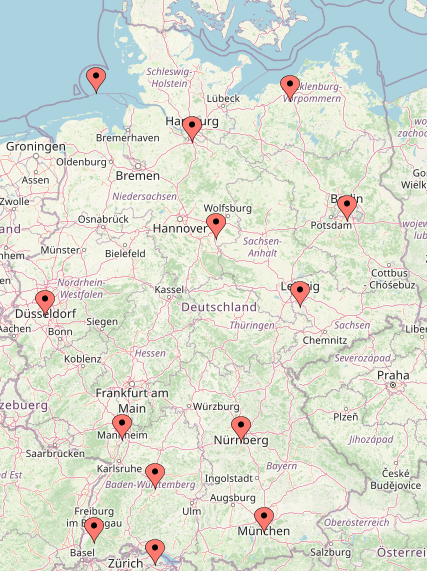
\includegraphics[width=.5\textwidth]{data/stations_map_customizer.png}
            \caption[Weather stations used]{Weather stations used}
            \label{fig::weather_stations}
 \end{figure}
 

\begin{table}[]
\begin{tabular}{l|l|l}
Station name & Measurements? & MOSMIX ?\\\hline
   Freiburg&Yes&Yes\\
   Hamburg&Yes&Yes\\
    Leipzig-Halle&Yes&Yes\\
    Nuernberg&Yes&Yes\\
    Stuttgart&Yes&Yes\\
    Mannheim&Yes&Yes\\
    Berlin-Tempelhof&Yes&Yes\\
    Duesseldorf&Yes&Yes\\
    Muenchen&Yes&Yes\\
   Konstanz&Yes&Yes\\
   Braunschweig&Yes&Yes\\
   Goettingen&Yes&Yes\\
   Rostock&Yes&Yes\\
   Helgoland&Yes&Yes   
\end{tabular}
\caption{Weather stations used for DWD data}
\label{Table::Weather_Stations}
\end{table}



 
 
% First explain concepts you used in your thesis like filters or methods
% Then explain your approach or algorithm
% Use flowcharts to give an overview

\section{Additional Data}
\label{Section::Additional_Data}
On top of these 3 major thematic fields additional information about working days was used. 

This data source is expected to capture variations in electricity load.
School holidays and extended weekends due to public holidays are typical times for taking vacations.
These effects will be analyzed later in the thesis.

\subsection{Holidays}

In germany there are static holidays which are always on the same day each year.
Examples for these are christmas or the 1st of may. 
Other holidays in germany are dependant on the date of easter. 
An example for such a holiday is the feast of ascension, which always happens 39 days after easter.

The bundesAPI provides an api to get information to get this information \cite{HolidayAPIUrl}.

\subsection{School Holidays}

Information about school holidays is provided by Schulferien.org \cite{SchoolHolidays}. 
The data is displayed in a table on this website. 
A webscraper is used to get the data.

\end{document}
